\section{Kết quả thử nghiệm hạ tầng sơ bộ}

Phần này trình bày kết quả thử nghiệm triển khai hạ tầng Kubernetes và các thành phần của hệ thống Florus trong giai đoạn Đồ án Chuyên ngành.

\subsection{Môi trường thử nghiệm}

\subsubsection{Cấu hình Cluster}

Môi trường thử nghiệm được thiết lập trên Minikube với cấu hình như sau:

\begin{table}[H]
\centering
\caption{Cấu hình Minikube Cluster}
\label{tab:minikube-config}
\begin{tabular}{|l|l|}
\hline
\textbf{Thông số} & \textbf{Giá trị} \\
\hline
Kubectl Client Version & v1.34.1 \\
\hline
Kubectl Server Version & v1.34.0 \\
\hline
Kustomize Version & v5.7.1 \\
\hline
Container Engine & v28.5.2 \\
\hline
CPU Allocation & 20 cores \\
\hline
Memory Allocation & 7.39 GB \\
\hline
Disk Allocation & 50 GB \\
\hline
Driver & Docker \\
\hline
CNI Plugin & Default \\
\hline
Ingress Controller & NGINX Ingress \\
\hline
\end{tabular}
\end{table}

\subsubsection{Addons được kích hoạt}

\begin{lstlisting}[caption={Minikube Addons}]
minikube addons enable ingress
minikube addons enable metrics-server
minikube addons enable dashboard
minikube addons enable storage-provisioner
\end{lstlisting}

\subsection{Kết quả triển khai thử nghiệm}

\subsubsection{Đã Deploy (Helm Chart: florus-platform + florus-infra + florus-monitor)}


\begin{table}[H]
    \centering
    \small 
    \renewcommand{\arraystretch}{1.2} 
    \begin{tabularx}{\textwidth}{@{}l l c X@{}}
        \toprule
        \textbf{Component} & \textbf{Pod Name Pattern} & \textbf{Svc Port} & \textbf{Mô tả \& Vai trò} \\
        \midrule
        
        % --- APPLICATION LAYER ---
        UI React & \texttt{florus-ui-*} & 80 & Frontend (Nginx) phục vụ giao diện người dùng SPA. \\
        
        API Gateway & \texttt{florus-api-gateway-*} & 5000 & Entrypoint trung tâm, định tuyến request và xác thực JWT. \\
        
        Auth Service & \texttt{florus-auth-service-*} & 8000 & \textit{(Container: 5005)} Dịch vụ xác thực và cấp phát Token. \\
        
        Ingestion Svc & \texttt{florus-service-ingestion-*} & 8001 & \textit{(Container: 5020)} Xử lý upload file và luồng dữ liệu thô. \\
        
        Delta Service & \texttt{florus-service-delta-*} & 8002 & \textit{(Container: 5015)} Quản lý thao tác đọc/ghi trên Delta Lake. \\
        
        % --- INFRA LAYER ---
        Spark Operator & \texttt{florus-spark-operator-*} & - & Controller quản lý vòng đời ứng dụng Spark (CRDs). \\
        
        MongoDB & \texttt{florus-infra-mongodb-*} & 27017 & NoSQL Database lưu trữ metadata và cache. \\
        
        MinIO & \texttt{florus-infra-minio-*} & 9000 & Object Storage lưu trữ Data Lake. \\
        
        % --- MONITORING LAYER ---
        Prometheus & \texttt{prometheus-florus-...-0} & 9090 & Time-series Database thu thập metrics hệ thống. \\
        
        AlertManager & \texttt{alertmanager-florus-...-0} & 9093 & Quản lý quy tắc và gửi cảnh báo. \\
        
        Grafana & \texttt{florus-monitor-grafana-*} & 3000 & Dashboard trực quan hóa dữ liệu giám sát. \\
        
        Node Exporter & \texttt{...-node-exporter-*} & 9100 & Agent thu thập thông số phần cứng (CPU/RAM) từng Node. \\
        
        \bottomrule
    \end{tabularx}
    \caption{Danh sách các thành phần đã triển khai và Cổng dịch vụ  tương ứng}
    \label{tab:deployed}
\end{table}

\begin{figure}[H]
    \centering
    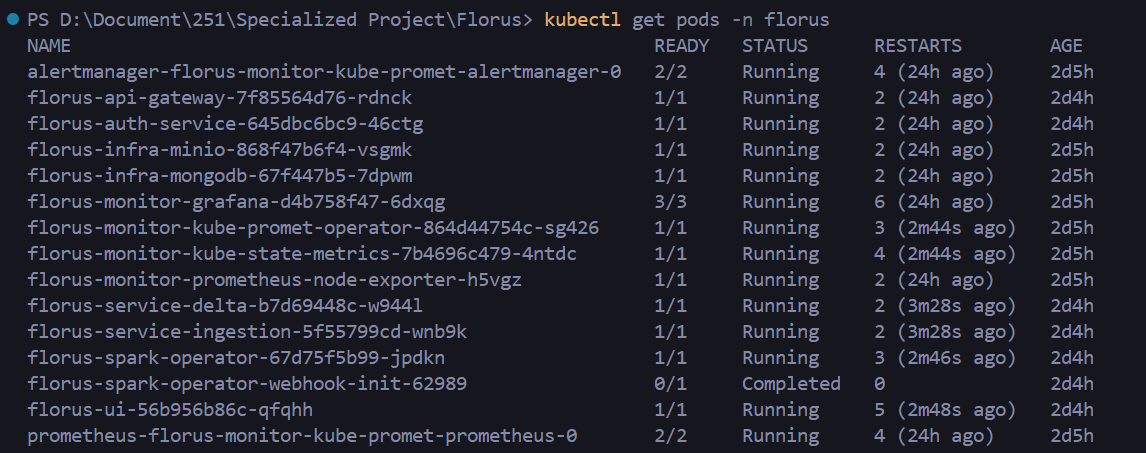
\includegraphics[width=0.95\linewidth]{images/chap 3/pods.png}
    \vspace{2em}
    \caption{Các pod của hệ thống đã được triển khai}
\end{figure}

\begin{figure}[H]
    \centering
    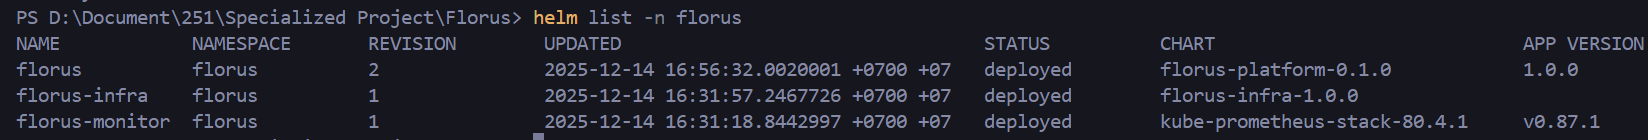
\includegraphics[width=0.95\linewidth]{images/chap 3/helm-list.png}
    \vspace{2em}
    \caption{Các helm release của hệ thống đã được triển khai}
\end{figure}

\begin{figure}[H]
    \centering
    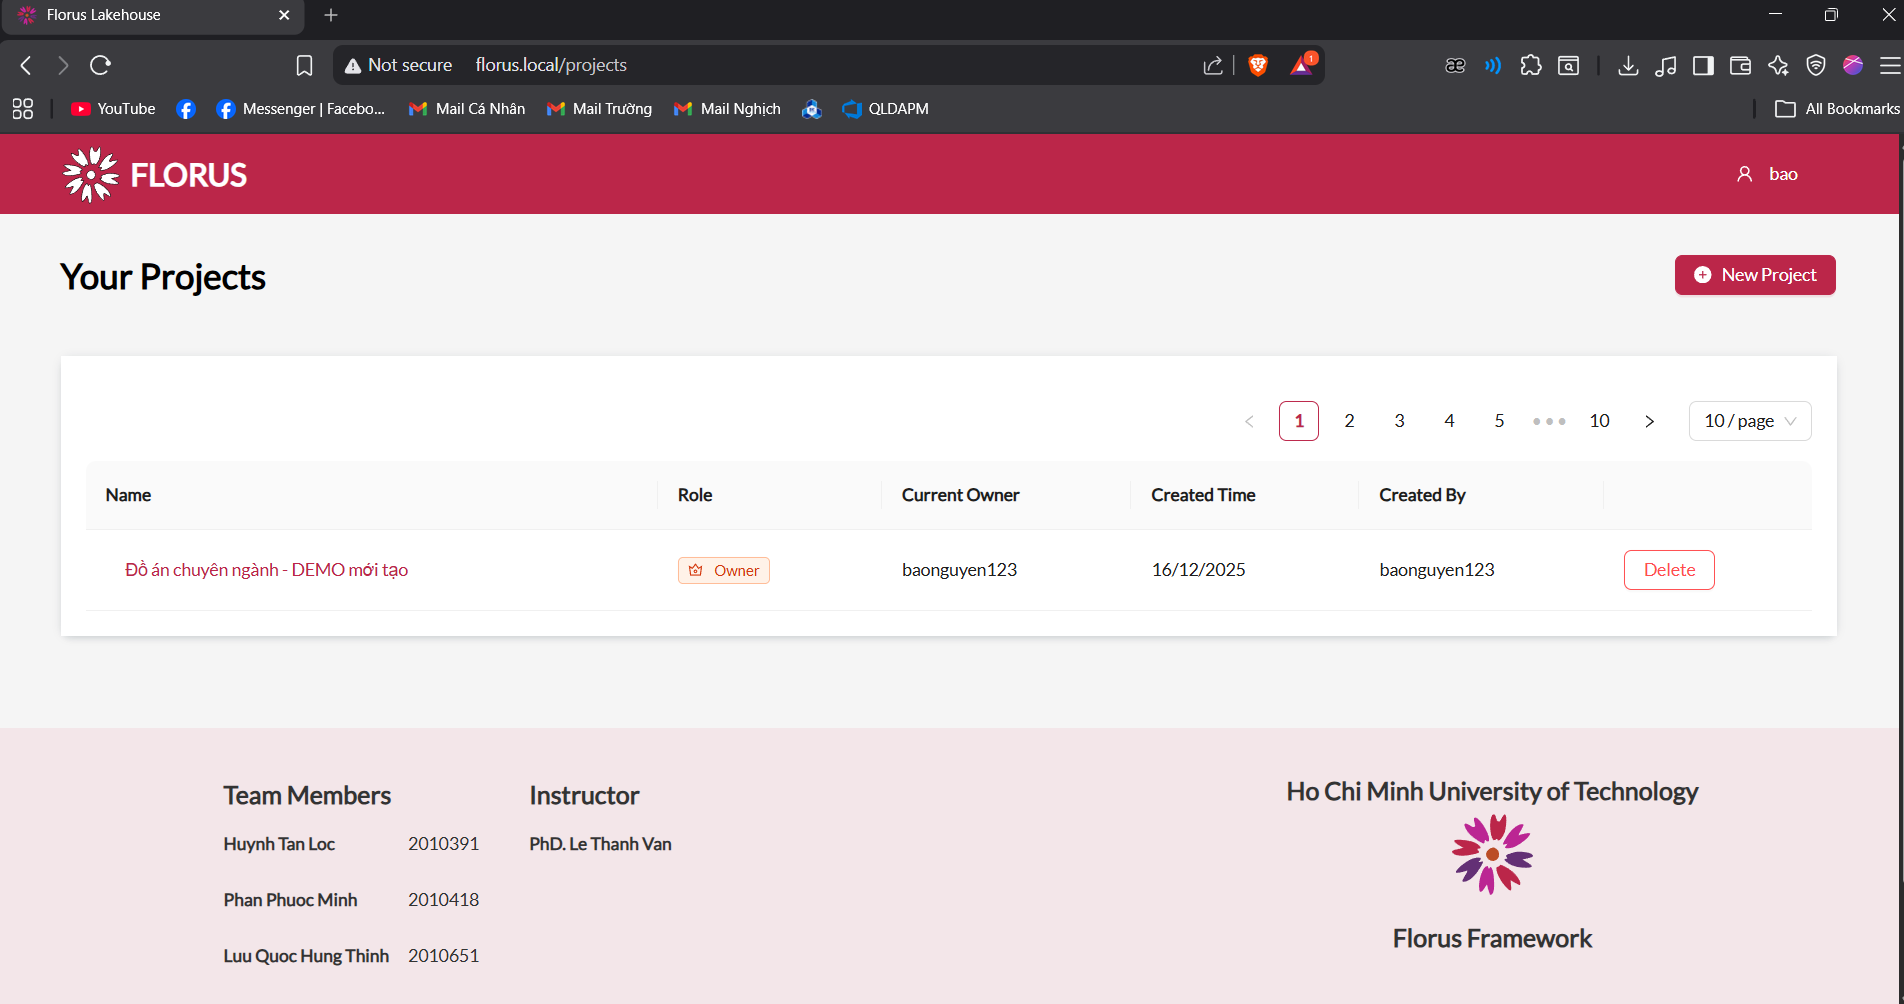
\includegraphics[width=0.95\linewidth]{images/chap 3/florus-ui.png}
    \vspace{2em}
    \caption{UI quản lý hệ thống đã có thể truy cập và tương tác}
\end{figure}

\subsubsection{Chưa Deploy (Cần tạo Helm chart)}

\begin{table}[H]
    \centering
    \small % Dùng font nhỏ hơn một chút để vừa vặn đường dẫn dài
    \renewcommand{\arraystretch}{1.3} % Tăng khoảng cách dòng cho thoáng
    
    % Định nghĩa lại cột Y để canh trái và tự xuống dòng (cho đẹp hơn X mặc định)
    \newcolumntype{Y}{>{\raggedright\arraybackslash}X}

    % Cấu trúc: 
    % l: Component (cố định)
    % l: Source Folder (cố định)
    % c: Port (giữa)
    % Y: Mô tả (co giãn)
    % Y: Dependencies (co giãn)
    \begin{tabularx}{\textwidth}{@{} l l c Y Y @{}}
        \toprule
        \textbf{Component} & \textbf{Source Folder} & \textbf{Port} & \textbf{Mô tả} & \textbf{Dependencies} \\
        \midrule
        
        Model Service & \texttt{service-model/} & 5025 & ML training với Spark MLlib & Mongo, MinIO, Spark \\
        
        Serving Service & \texttt{service-serving/} & 5030 & Model inference API & Mongo, MinIO \\
        
        Visualization Service & \texttt{service-visualization/} & 5035 & Chart generation & MongoDB \\
        
        Kafka Cluster & \texttt{kafka-cluster-kraft-local/} & 9092 & Event streaming & - \\
        
        MLflow & \texttt{mlflow\_with\_minio/} & 5000 & Experiment tracking & PostgreSQL, MinIO \\
        \bottomrule
    \end{tabularx}
    \caption{Các thành phần chờ triển khai trong hệ thống}
    \label{tab:undeployed}
\end{table}

% \subsubsection{Kiểm tra kết nối giữa các thành phần}

% \begin{itemize}
%     \item \textbf{API Gateway $\rightarrow$ Backend Services:} Thành công. Request được route đúng đến các service tương ứng.

%     \item \textbf{Services $\rightarrow$ MongoDB:} Thành công. Kết nối qua CoreDNS với hostname \texttt{mongodb.florus-infra.svc.cluster.local}.

%     \item \textbf{Ingestion Service $\rightarrow$ Kafka:} Thành công. Producer có thể gửi message vào topic \texttt{test-events}.

%     \item \textbf{Delta Service $\rightarrow$ MinIO:} Thành công. Đọc/ghi object qua S3 API.
% \end{itemize}

\subsection{Đánh giá Helm Charts}

\subsubsection{Cấu trúc Umbrella Chart}

Việc tổ chức Helm Charts theo mô hình phân tầng đã được kiểm chứng:

\begin{lstlisting}[caption={Cấu trúc Helm Charts}]
k8s/
+-- infra/          # Infrastructure Layer
|   +-- Chart.yaml
|   +-- values.yaml
|   +-- templates/
+-- florus-platform/       # Platform Layer
|   +-- Chart.yaml
|   +-- values.yaml
|   +-- charts/
|       +-- api-gateway/
|       +-- auth-service/
|       +-- ...
+-- monitoring/     # Monitoring Layer
|   +-- spark-pod-monitor.yaml (Prometheus được cài đặt riêng trong script deploy)
+-- deploy.ps1
\end{lstlisting}

\subsubsection{Kết quả triển khai bằng Helm}

\begin{lstlisting}[caption={Lệnh triển khai Helm}]
# Deploy Infrastructure
helm upgrade --install florus-infra ./florus-infra \
    -n florus-infra --create-namespace

# Deploy Platform
helm upgrade --install florus-platform ./florus-platform \
    -n florus-platform --create-namespace \
    -f values-dev.yaml

# deploy toàn hệ thống (rollout hoặc tạo mới hoàn toàn)
.\deploy.ps1 
\end{lstlisting}

Kết quả:
\begin{itemize}
    \item Thời gian triển khai toàn bộ hệ thống: 3 đến 5 phút nếu đã có sẵn các image và các image được load vào môi trường minikube; dạo động 10 đến 20 phút nếu tạo mới từ đầu (thời gian tải nhiều tài nguyên + thời gian build các image).
    \item Không có lỗi template rendering
    \item Tất cả Pods đạt trạng thái Running
    \item ConfigMaps và Secrets được tạo đúng
\end{itemize}

\clearpage
\newgeometry{top=0cm, bottom=0cm, left=4cm, right=0cm} % Ép lề nhỏ lại chỉ cho trang này
\begin{landscape}
    \thispagestyle{plain} % Bỏ Header "Đồ án...", chỉ giữ số trang ở dưới footer (tùy chọn)
    
    \begin{figure}[H]
        \centering
        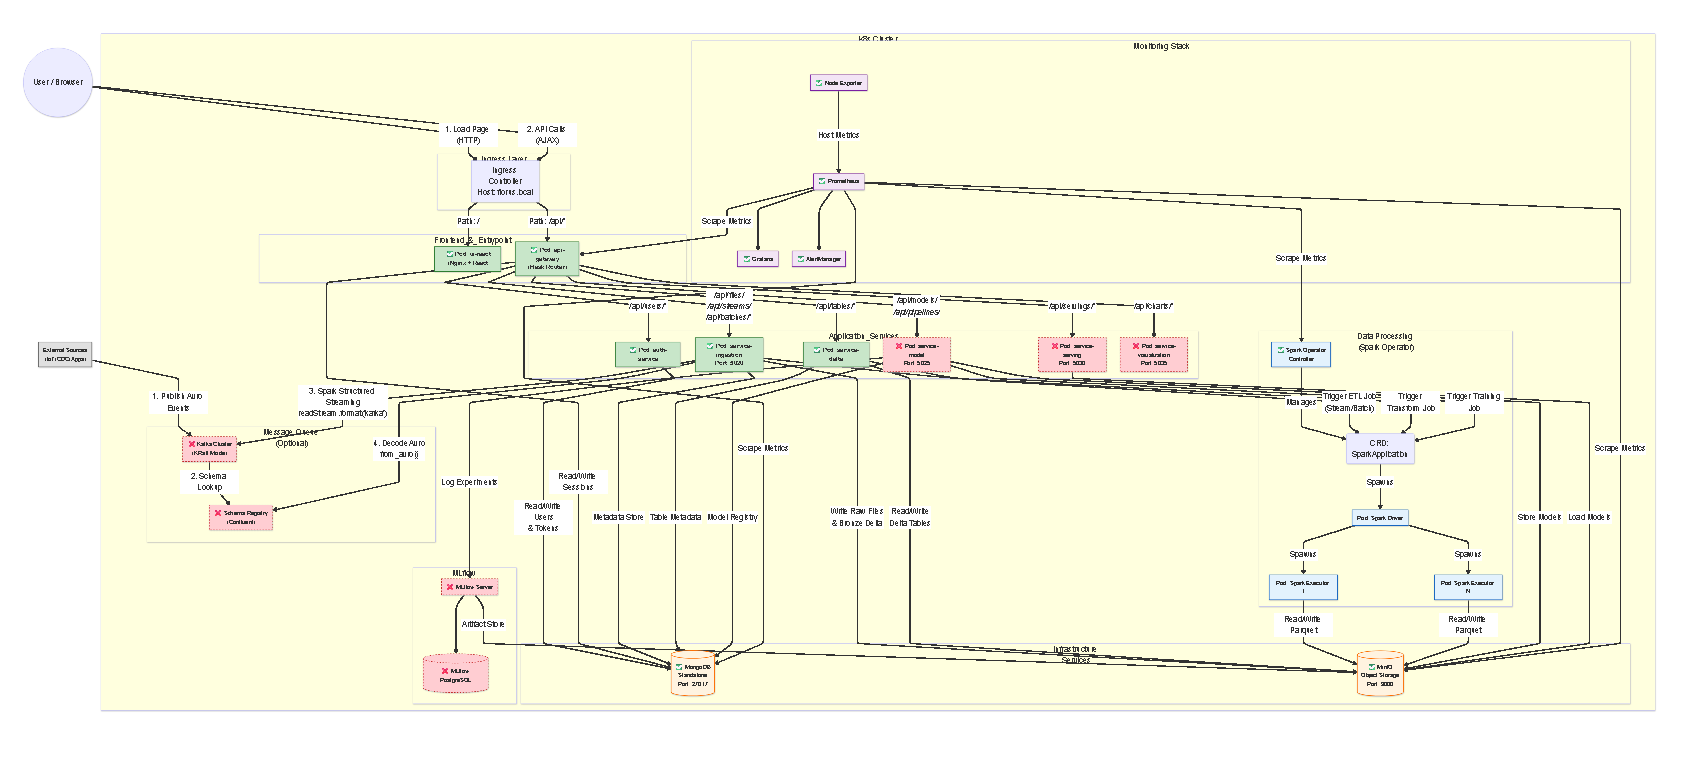
\includegraphics[width=1.0\linewidth, height=1.0\textheight, keepaspectratio]{images/chap 3/florus-full-lr (1).pdf}
        \caption{Kiến trúc triển khai hệ thống Florus trên nền tảng Kubernetes}
        \label{fig:florus-arch}
    \end{figure}
\end{landscape}
\restoregeometry % Trả lại lề chuẩn cho các trang sau
\clearpage



\subsection{Các vấn đề gặp phải và giải pháp}

\begin{table}[H]
\centering
\caption{Các vấn đề và giải pháp trong quá trình thử nghiệm}
\label{tab:issues-solutions}
\begin{tabular}{|p{5cm}|p{9cm}|}
\hline
\textbf{Vấn đề} & \textbf{Giải pháp} \\
\hline
Helm Release quá lớn (>1MB) & Phân tách thành 3 Charts riêng biệt (Infra, Platform, Monitoring) \\
\hline
Pod không resolve được DNS & Chờ CoreDNS khởi động hoàn tất, thêm initContainer để check DNS \\
\hline
MinIO S3 path style & Cấu hình \texttt{s3.path.style.access=true} trong Spark config \\
\hline
Resource không đủ & Giảm resource requests cho môi trường dev (chỉ cấu hình 1 replica cho mỗi service/DB)\\
\hline
\end{tabular}
\end{table}

\subsection{Kết luận thử nghiệm}

Kết quả thử nghiệm chứng minh tính khả thi của việc chuyển đổi hệ thống Florus sang Kubernetes:

\begin{enumerate}
    \item \textbf{Helm Charts hoạt động đúng:} Mô hình Umbrella Chart với phân tầng (Infra/Platform/Monitoring) giải quyết được vấn đề quản lý và giới hạn kích thước release.

    \item \textbf{Service Discovery qua DNS:} CoreDNS thay thế hoàn toàn file \texttt{/etc/hosts}, các services giao tiếp qua DNS names ổn định.

    \item \textbf{MinIO thay thế HDFS:} S3-compatible API hoạt động tốt với Spark và các services khác.

    \item \textbf{Declarative Deployment:} Toàn bộ hệ thống có thể được triển khai/hủy bằng một lệnh Helm.
\end{enumerate}

Các kết quả này là nền tảng để tiến hành giai đoạn Đồ án Tốt nghiệp với việc triển khai tiếp các service còn lại, bên cạnh đó tích hợp thêm AI Model và triển khai trên môi trường Production với multi-node cluster.
